%!TEX root = ../crimson_throne_book_main.tex
% 2015-08-22
While making their way to the temple of Aroden, the companions find the streets mostly abandoned. Has the plague decimated this district so thoroughly that there is hardly anyone left or are people so scared of the emperor that they dread coming outside? The first reason will surely have a huge impact, but fear of Pilts Swastel definitely plays a part as well, which becomes clear by the little game some ragged children are playing. Faking an execution with some simple wooden stick dolls and guillotine, the kids sing a macabre song:\\

"Off with your head, off with your head!   Sjo tries to scare away the children by telling them he will grow two heads if his is ever chopped off, but these little upstarts are not spooked easily. Having survived as long as they have in these inhuman circumstances has clearly hardened them. They simply change their lyrics to "off with your heads The temple of Aroden is an old, crumbling building which has lost almost all of its former splendor. Sjo uses a new neat trick and summons a pair of fiery wings, allowing him to fly up to the bell tower. Using his mace, he strikes the brass bell in an effort to distract whoever is inside the building, while his friends burst through the front doors. The ring of the bell is answered by the rattling of chains and the wails of a young child crying out in pain. When Balian pushes open the front doors, he finds the temple covered in a web of chains. A strange figure, dressed in tattered robes, is standing at the other end of the room. Multiple chains flow from his body and seem to bring the entire iron meshwork to life. Above the altar hangs the squirming form of Korwick. The shackles are squeezing him ever tighter and make him scream out in agony. Balian and Quint find a path through the tangled web and close in on the enemy, who unleashes a cacophony of dark, soul-shaking howls from the pits of hell. A pitch-black cloud spreads out around him and the overwhelming scream deafens the two brave heroes, who summon the strength of their will to fight back an even nastier effect. Puk and Sjo enter as well, but the Shoanti is the only one who can see in the dark - his limited {\itshape clouded vision} does have its advantages after all. He notices that the evil fiend moves through the sea of iron braids with ease, while his friends all get caught in it. The healer throws a  {\itshape burning hands} on the creature, but the flames simply glide off its body, leaving it unharmed. Spyder's keen sense of smell allows the dog to locate the devilish monster in the darkness and attack it with a  {\itshape critical} bite. But the canine's teeth do almost no damage. So the devil needs specific weapons to be hurt; unfortunately no one in the party possesses the knowledge to know which. Groping around in the blackness and struggling with the entangling chains makes the party very inefficient. Balian manages to pull free from the grasp of the web and makes his way to the monster, but as the darkness drops away, he now faces the  {\itshape unnerving gaze} of the sacristan kyton - who has lowered his hood - and is staggered. The chain devil keeps moving agilely through the crisscross of strings and lashes out mercilessly with his own spiked chain, making all the heroes bleed. Quint stumbles out of the church and pull out his wand of  {\itshape feather step} to allow himself faster movement in this difficult terrain. \hyperref[fig:Chain-devil-in-the-temple-of-Aroden-555419466]{ The combination of the entangling chains and the unsettling eyes of the kyton make this fight very hard. } The companions keep getting stuck in the iron web - even the dexterous rogue Puk - and the monster's gaze continually steals actions from the heroes if they fail to summon the willpower to resist. The only upside is that the devil's most efficient tactic is to cleave away at his enemies, thus spreading the damage over multiple targets, instead of focus firing. Of course, this forces the companions into combat healing as well, Puk has to pull out a potion to stay in the fight, while Quint resorts to his  {\itshape wand of cure serious wounds} and Sjo burns through his own healing magic. Quint makes it to the altar, where the strangling chains have forced poor Korwick into unconsciousness. He saves the boy's life with a touch of the wand. Meanwhile Balian scores his first hit; his greatsword's magic is not empowered to bypass the devil's damage reduction, but his heavy hit still deals a fair gash. The ranger's skill of following up when his enemy tries to step away also proves its worth, forcing the devil to stop moving about. Sjo also closes in on the kyton and strikes hard twice. It takes many more rounds of healing, striking and trying to avoid the creature's gaze or facing the potential staggering effect before Puk finally gets into position and finds that the silver of his off-hand short sword actually does full damage to the fiend. The halfling's first strike is also his last, as the sacristan kyton finally drops to the floor, defeated at last. \\

\begin{figure}[h]
	\centering
	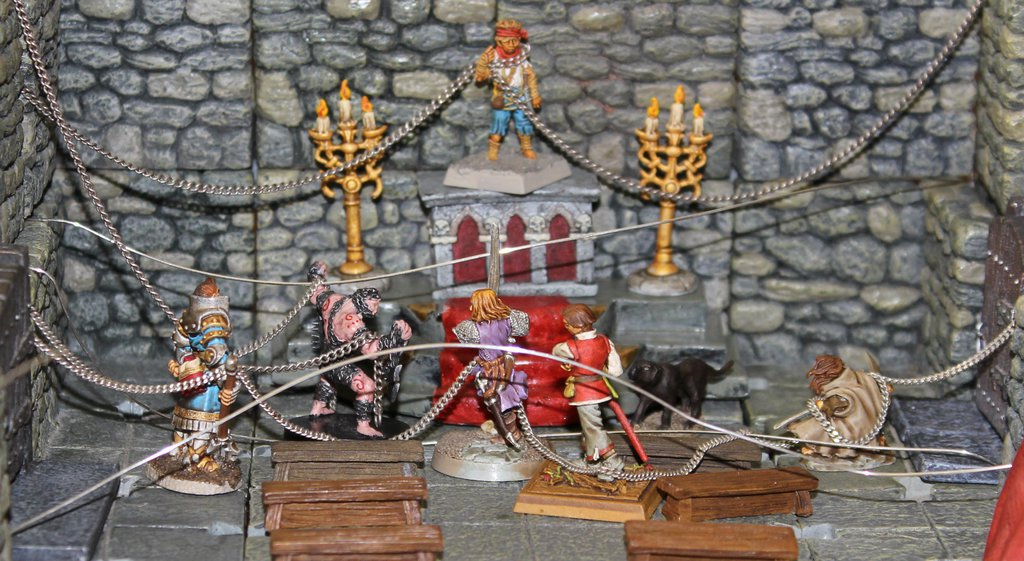
\includegraphics[width=0.39\textwidth]{images/Chain-devil-in-the-temple-of-Aroden-555419466.jpg}
	\caption{Chain devil in the temple of Aroden}
	\label{fig:Chain-devil-in-the-temple-of-Aroden-555419466}
\end{figure}

The companions dig deeply into their resources of healing wands to restore everyone to full health. Korwick has lost consciousness again, but is still alive! Puk finds another wooden miniature building, representing the Copper-Beater hall, an enterprise close to the pier of Eel's End. This wooden toy house fits the feet of the Heldrin puppet. Sjo also discovers the bodies of the three priests of Aroden in a backroom of the temple. They have all been slashed to death by the kyton's cruel barbs.\\

